\chapter{Documentation}
\label{chap:num_8}

The following chapter provides the information on available documentation resources implemented for both \lpas{} package and \lpa{} Storage Components. Selected code snippets demonstrate the core usage and provide detailed references for hosted documentations. The first section will start with user documentation covering a generic interaction flow with \lpa{} platform using \lpas{} package and React Storage Components. The remaining sections will dive deeper into the developer documentation. Starting from the installation guide and documentation of \lpa{} package hosted on GitHub Pages and finalizing at an overview of how \lpa{} Storage Components were integrated into documentation resources of \lpa{} platform.

\section{User documentation}
\label{sssec:user_documentation_guides}

This section is intended for non-developers who want to evaluate and try out the latest release of \lpa{} platform with integrated \lpas{} package and \lpa{} Storage Components implemented. The documentation will serve as a tutorial expanding a generic user story first introduced in \autoref{fig:lpa_user_story}. To recap, we have two target platform users named John and Bob. John attempts to use \lpa{} platform, create and publish the application. On the other hand, Bob wants to see the resulting application created and shared by John. The documentation will cover interactions with a live instance of the latest \href{https://applications.linkedpipes.com}{\lpa{} release}, hosted at the Software Engineering department at Faculty of Mathematics and Physics in Charles University.
The user-story based guideline will focus mainly on \lpas{} and \solid{} related aspects, therefore for more specific information regarding other \lpa{} platform features refer to the official user documentation \footnote{\url{https://docs.applications.linkedpipes.com}} of the platform. 

\subsection{Creating Account}

The first step for John is to create his first \solid{} POD and associated WebID profile. Referring back to \autoref{sssec:user_authentication_implementation} and \autoref{fig:lpa_login_webpage}, after selecting a provider, for instance LinkedPipes PODs, he will be redirected to a \solid{} server login webpage demonstrated at \autoref{fig:solid_login_webpage}, where a \textit{Create an account} button needs to be clicked. After that he will be redirected to a \solid{} server signup webpage demonstrated at \autoref{fig:solid_login_webpage}. Lastly after creating a \solid{} account he will be redirected to a his POD webpage. Performing the login at \lpa{} instance website will now be possible with John's new WebID and \solid{} POD created under selected provider.

\begin{figure}[h]
\centering
\fcolorbox{black}{white}{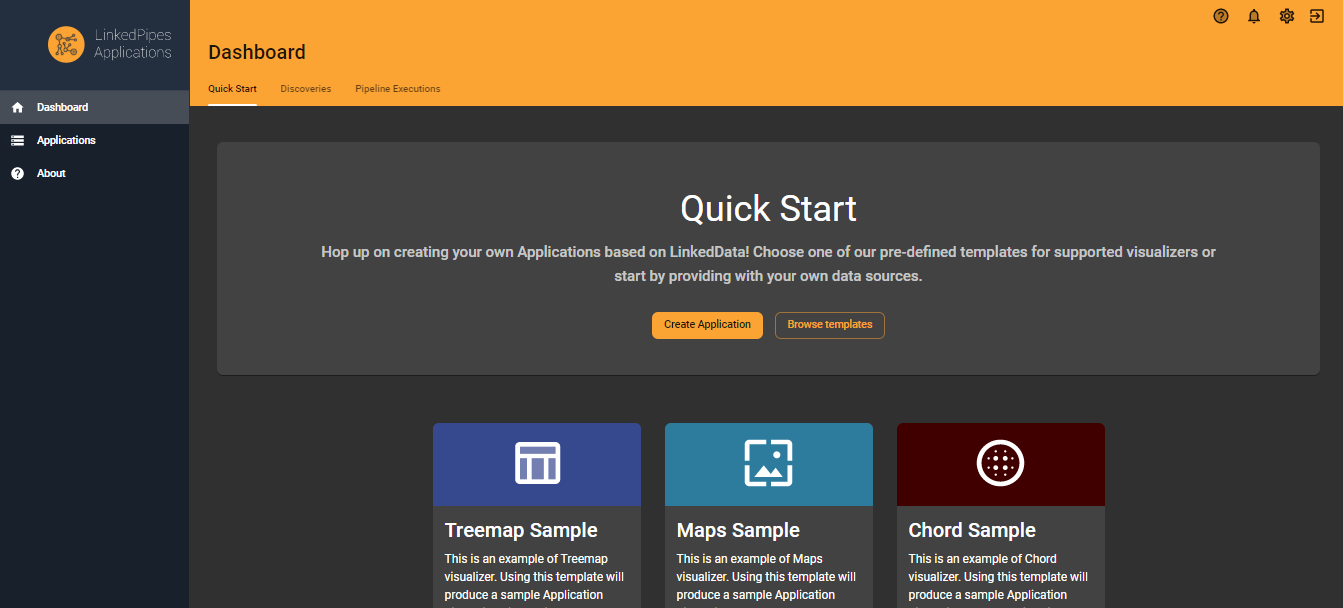
\includegraphics[width=0.8\linewidth]{dashboard.png}}
\caption{The Dashboard page displayed after successfull authentication into \lpa{} platform.}
\label{fig:dashboard}
\end{figure}

After successfull authentication an \lpa{} Dashboard page demonstrated on \autoref{fig:dashboard} will be presented. 

\subsubsection{Notes for providers using the latest NSS versions}

One distinct difference in NSS releases starting from the fifth version, and higher is more strict access control settings when authenticating a \solid{} application with a \solid{} POD. Since the majority of stable features of \lpas{} were developed before under fourth release iteration of NSS, it was impossible to simplify the authentication flow for the newer version due to constant changes and updates in both NSS releases and \solid{} specifications. Therefore, for \lpa{} users that are intended to use the providers that supply \solid{} servers based on the latest NSS version, there is one additional manual step required during initial signup. As demonstrated on \autoref{fig:lpa_solid_authorize}, this popup will be displayed during the initial login to \lpa{} platform after creating a \solid{} account, it is crucial to enable the \textit{Give other people, and apps access to the Pod, or revoke their (and your) access} option. This will ensure that the \solid{} app will have enough privileges to create and edit the ACL files associated with visualizer configurations inside the POD. 

\begin{figure}[h]
\centering
\fcolorbox{black}{white}{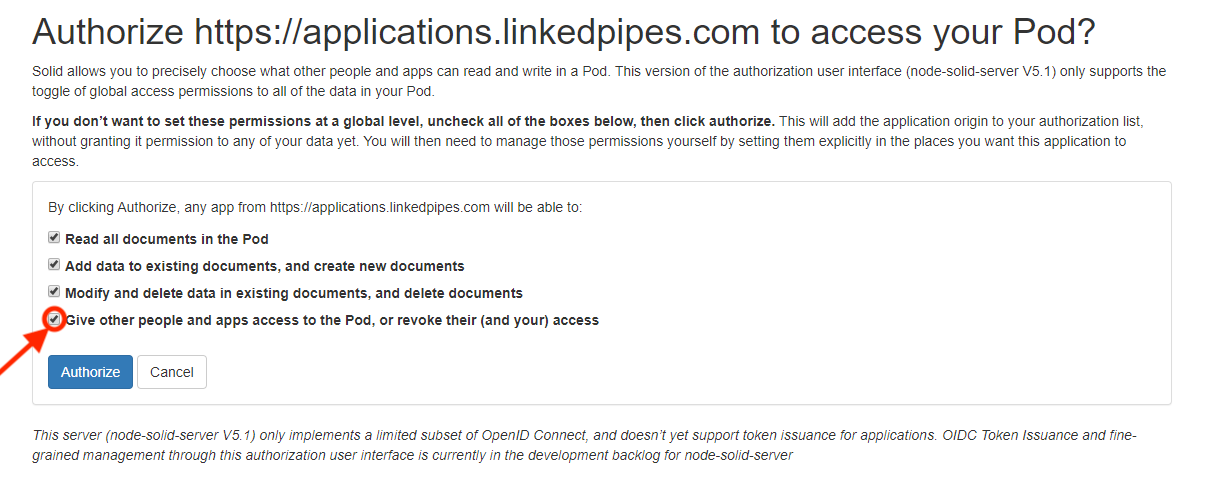
\includegraphics[width=0.8\linewidth]{lpa_solid_authorize.png}}
\caption{An access control popup displayed on latest NSS instances.}
\label{fig:lpa_solid_authorize}
\end{figure}

\subsection{Creating Application}

To create an application, John must either provide the necessary data source information or select one of the data sample templates provided at the Dashboard page.

To use one of the data samples provided by \lpa{}, on the Dashboard page, John needs to click the \textit{Choose} button on the desired data sample template. This will redirect him the Create Application page, as displayed on \autoref{fig:create_app}, where the data source fields will already be pre-filled, and he can proceed to click \textit{Start Discovery} immediately. In this guide, it is assumed that John started the application creation process using templates. For more details on other ways to provide data sources, refer to the official \lpa{} platform documentation.

\begin{figure}[h]
\centering
\fcolorbox{black}{white}{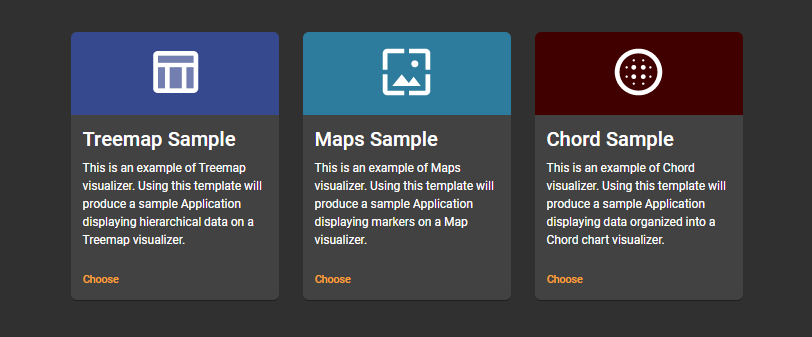
\includegraphics[width=0.8\linewidth]{data_samples.png}}
\caption{Template data sources provided by \lpa{} platform.}
\label{fig:data_samples}
\end{figure}

\begin{figure}[h]
\centering
\fcolorbox{black}{white}{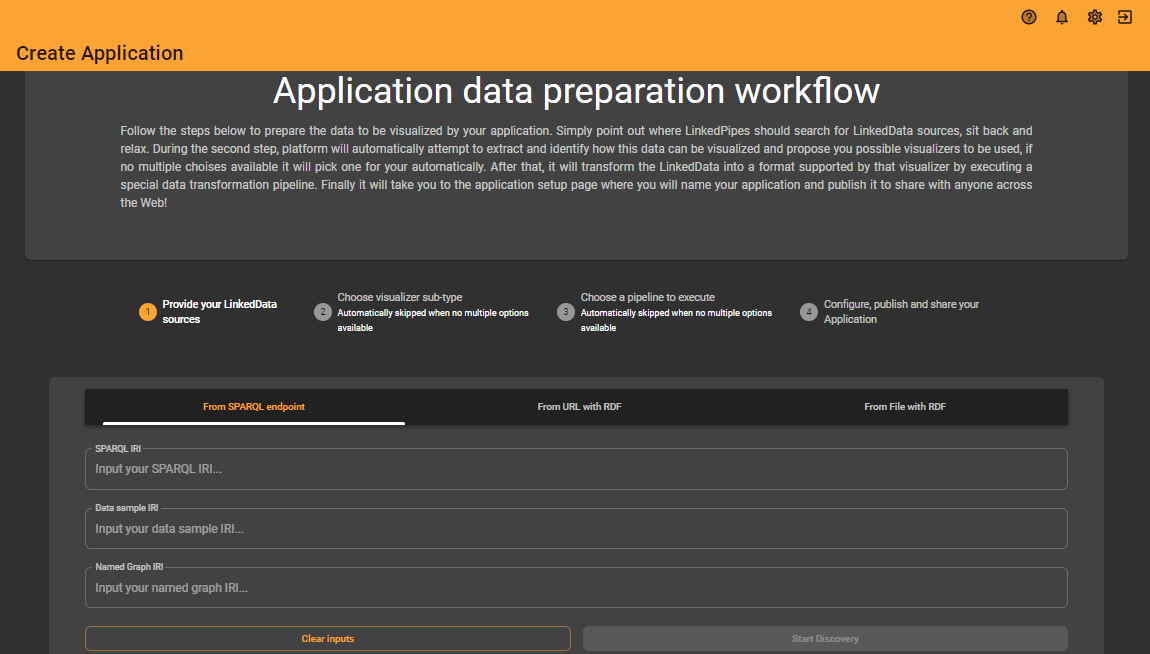
\includegraphics[width=0.8\linewidth]{create_app.png}}
\caption{Create Application page.}
\label{fig:create_app}
\end{figure}

After the discovery process finishes, the user will be prompted to pick one of the recommended visualizers, as displayed on \autoref{fig:choose-visualizer}. If only one possible visualizer is available, this step will be skipped as that visualizer will be automatically picked by \lpa{}.

\begin{figure}[h]
\centering
\fcolorbox{black}{white}{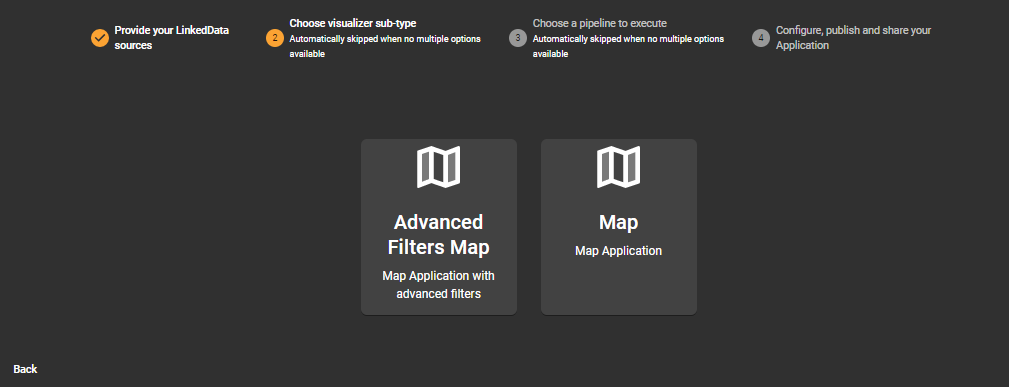
\includegraphics[width=0.8\linewidth]{choose_visualizer.png}}
\caption{Create Application page - Choose Visualizer.}
\label{fig:choose-visualizer}
\end{figure}

Clicking on the desired visualizer will trigger the data transformation process, as displayed on \autoref{fig:processing_pipeline}. In other words, the pipeline transformations will be applied to the whole RDF data based on the data sources given. If more than one applicable pipeline is found, John will be asked to choose one before this process begins.

The resulting data will then be in the format required to be visualized using the selected visualizer.

\begin{figure}[h]
\centering
\fcolorbox{black}{white}{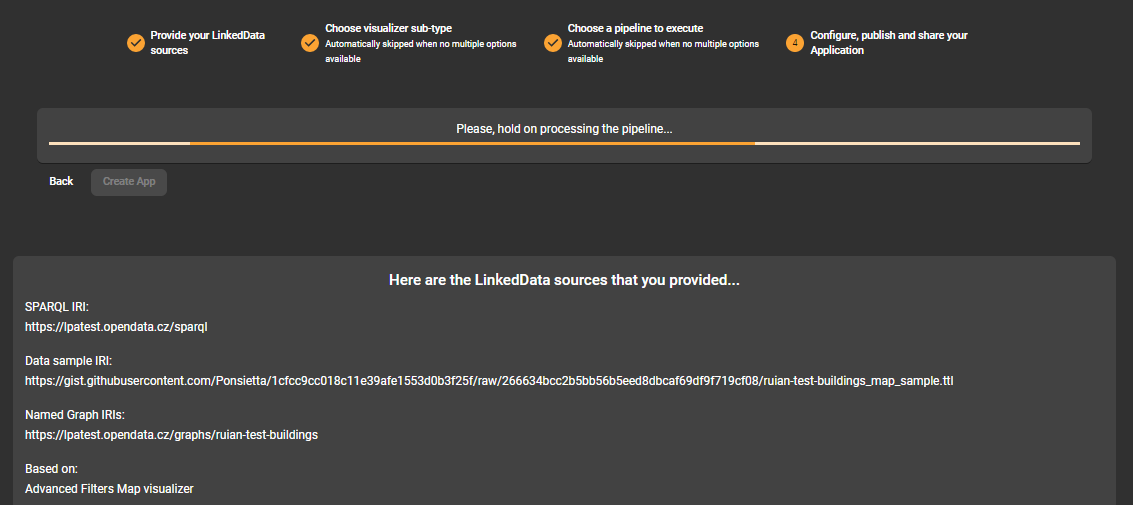
\includegraphics[width=0.8\linewidth]{processing_pipeline.png}}
\caption{Create Application page - Executing pipeline.}
\label{fig:processing_pipeline}
\end{figure}

Once this step is complete, as presented on \autoref{fig:finished_execution}, John can click on 'Create App' to visualize the data and customize the visualization on a separate webpage called \textit{Application Control and Setup}.

\begin{figure}[h]
\centering
\fcolorbox{black}{white}{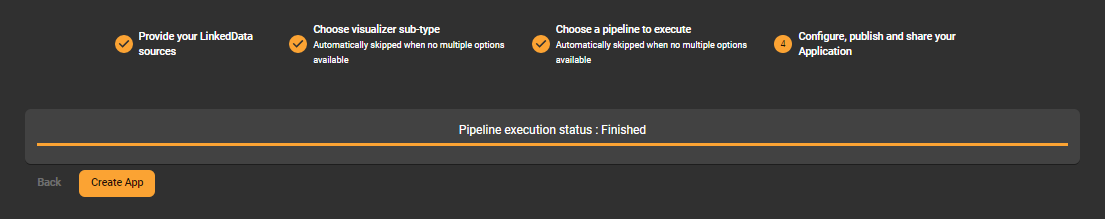
\includegraphics[width=0.8\linewidth]{finished_execution.png}}
\caption{Create Application page - Finished pipeline execution.}
\label{fig:finished_execution}
\end{figure}

\subsection{Publishing application}

As presented on \autoref{fig:create_application_screen}, the \textit{Application Control and Setup} page consists of the preview of the visualizer to be published, a set of controls to configure the filters (if available) and a header component with elements to publish or embed the application. To publish an application by storing the visualizer configuration in \solid{} POD, John needs to input the title for his application and click on the \textit{Publish} button. Alternatively he can click on \textit{Embed} application an will be presented with a simple popup to generate the HTML \texttt{iframe}. For more specific details on publishing and storing in \solid{} refer to the description in \autoref{sssec:create_store_and_publish_application}. For more specific details on configuring the post published application refer to \autoref{sssec:configuring_application_implementation}.

\begin{figure}[h]
\centering
\fcolorbox{black}{white}{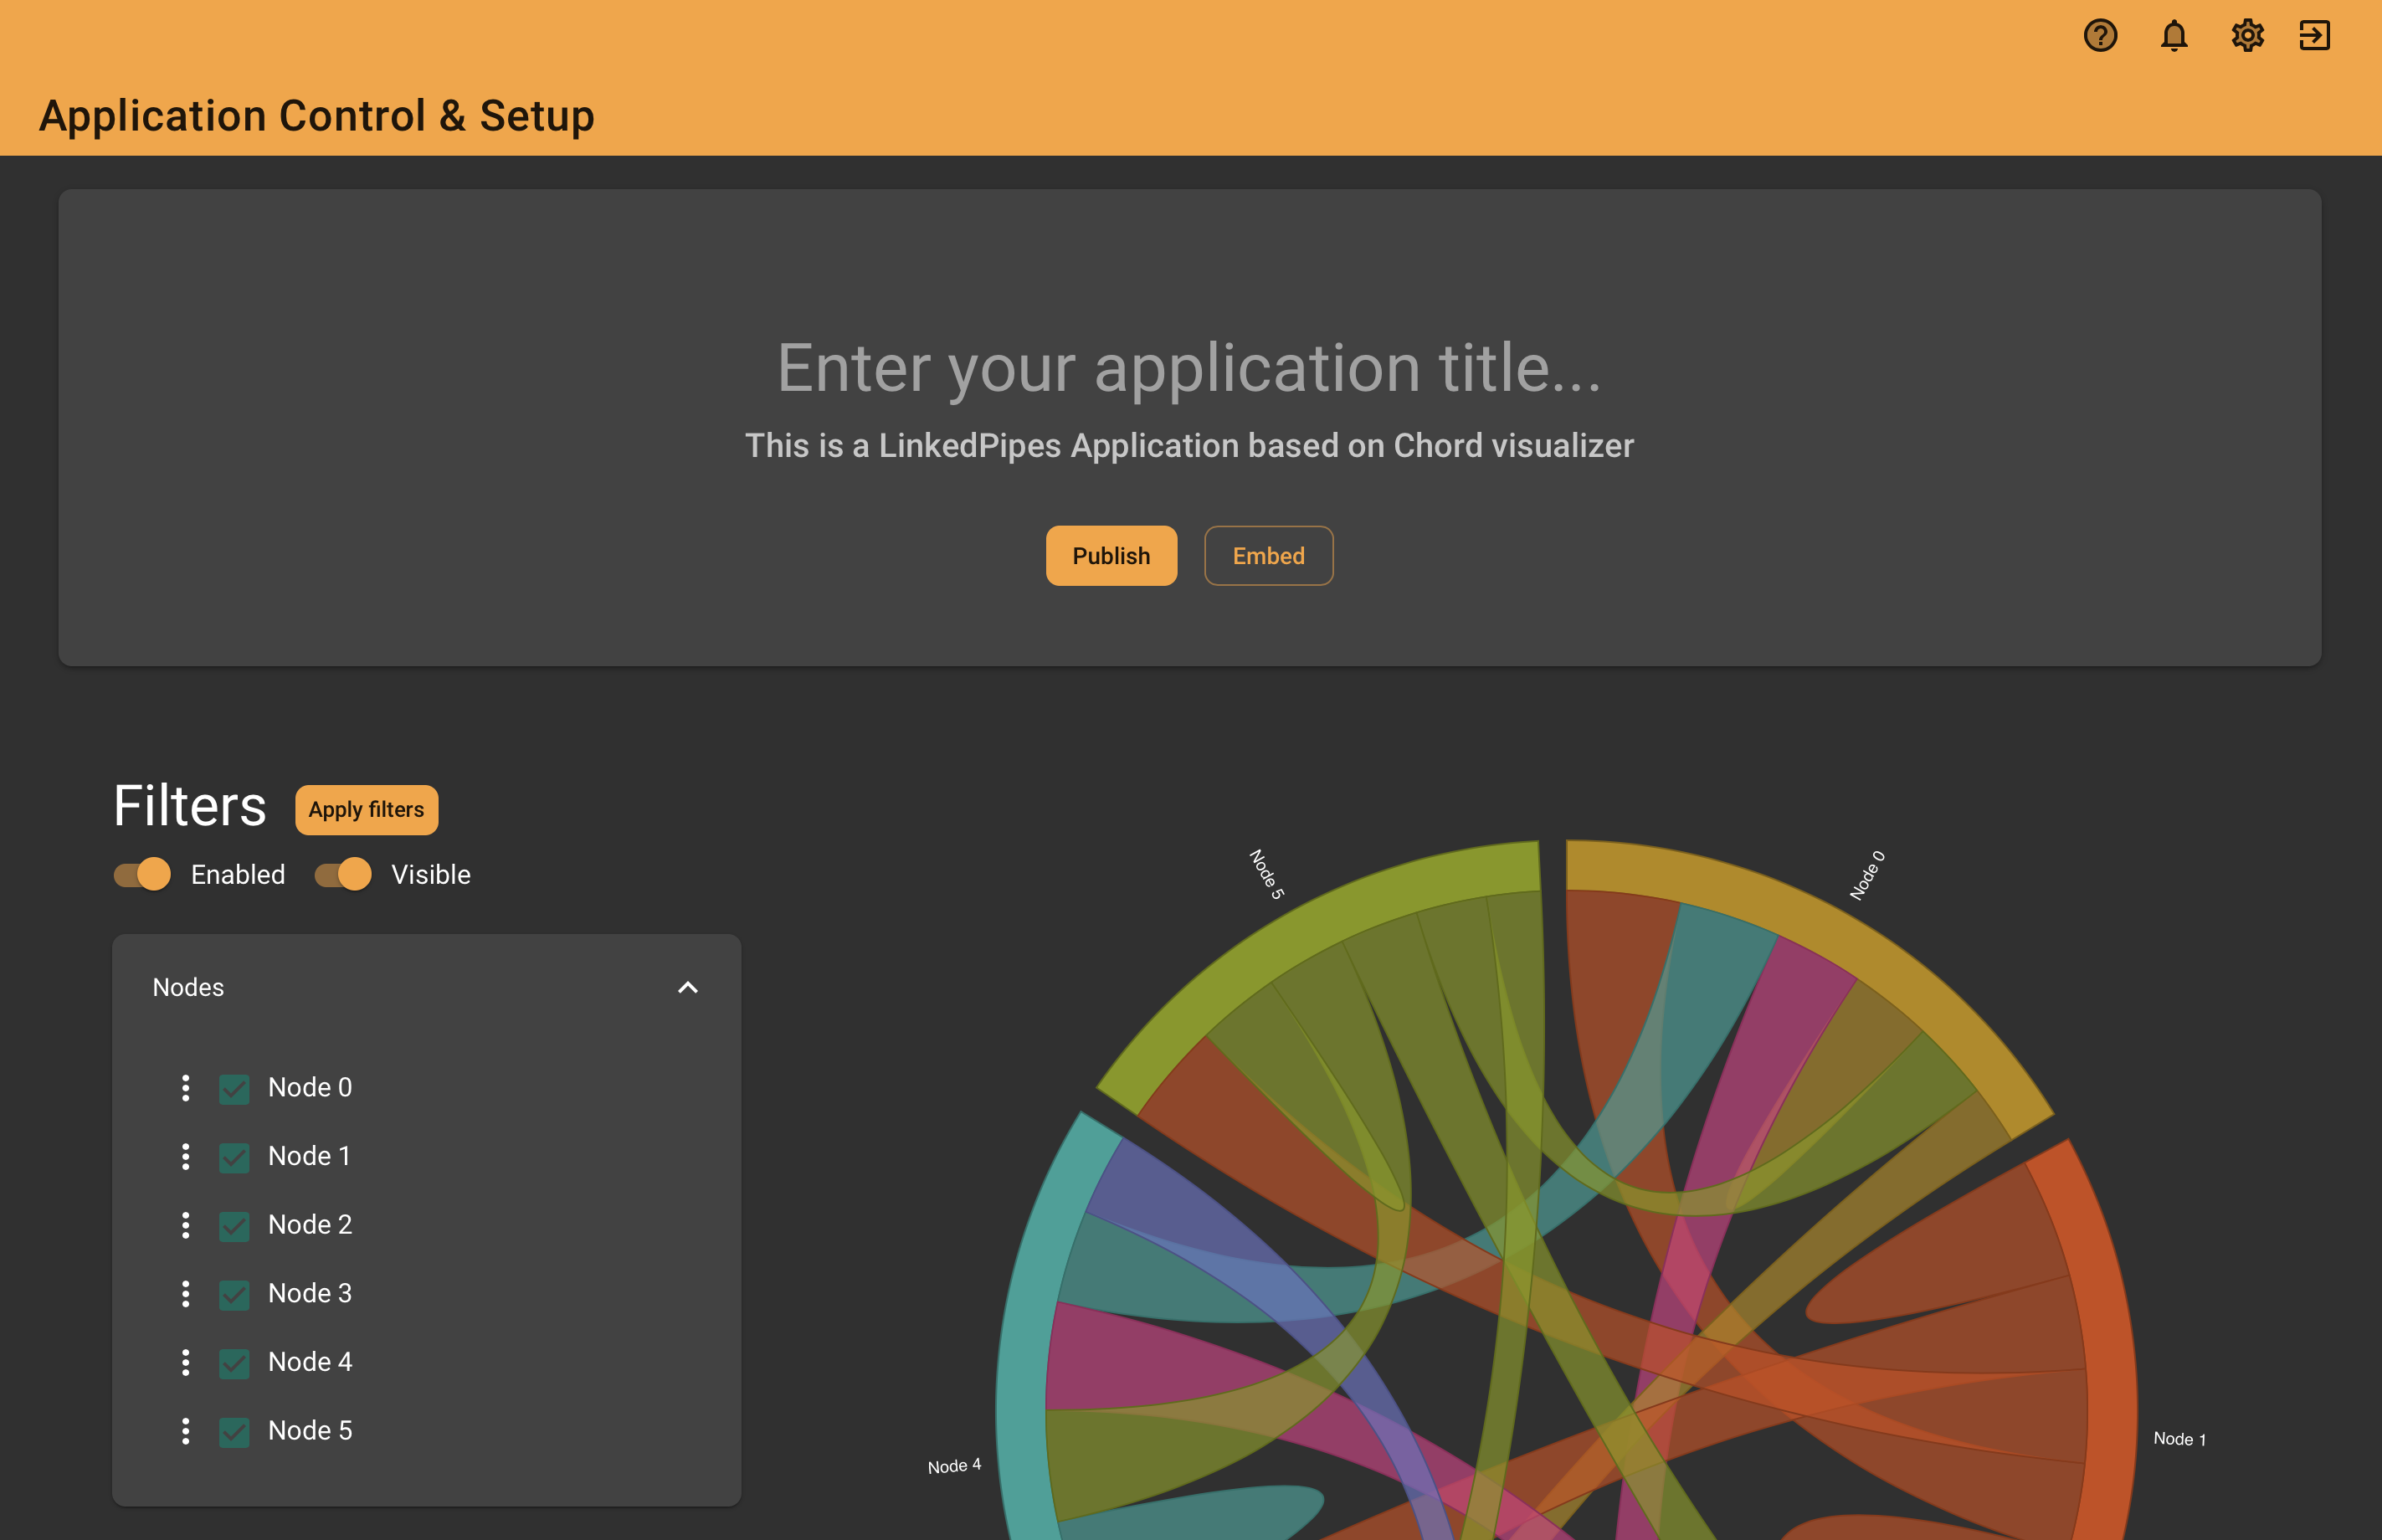
\includegraphics[width=0.8\linewidth]{create_application_screen.png}}
\caption{Application Control and Setup webpage.}
\label{fig:create_application_screen}
\end{figure}

The screenshot on \autoref{fig:solid_published_app_config} represents a webpage for the stored application configuration inside the \solid{} POD. Every published application configuration have their own URI that is used during the generation of a URL to share the visualization.

\begin{figure}[h]
\centering
\fcolorbox{black}{white}{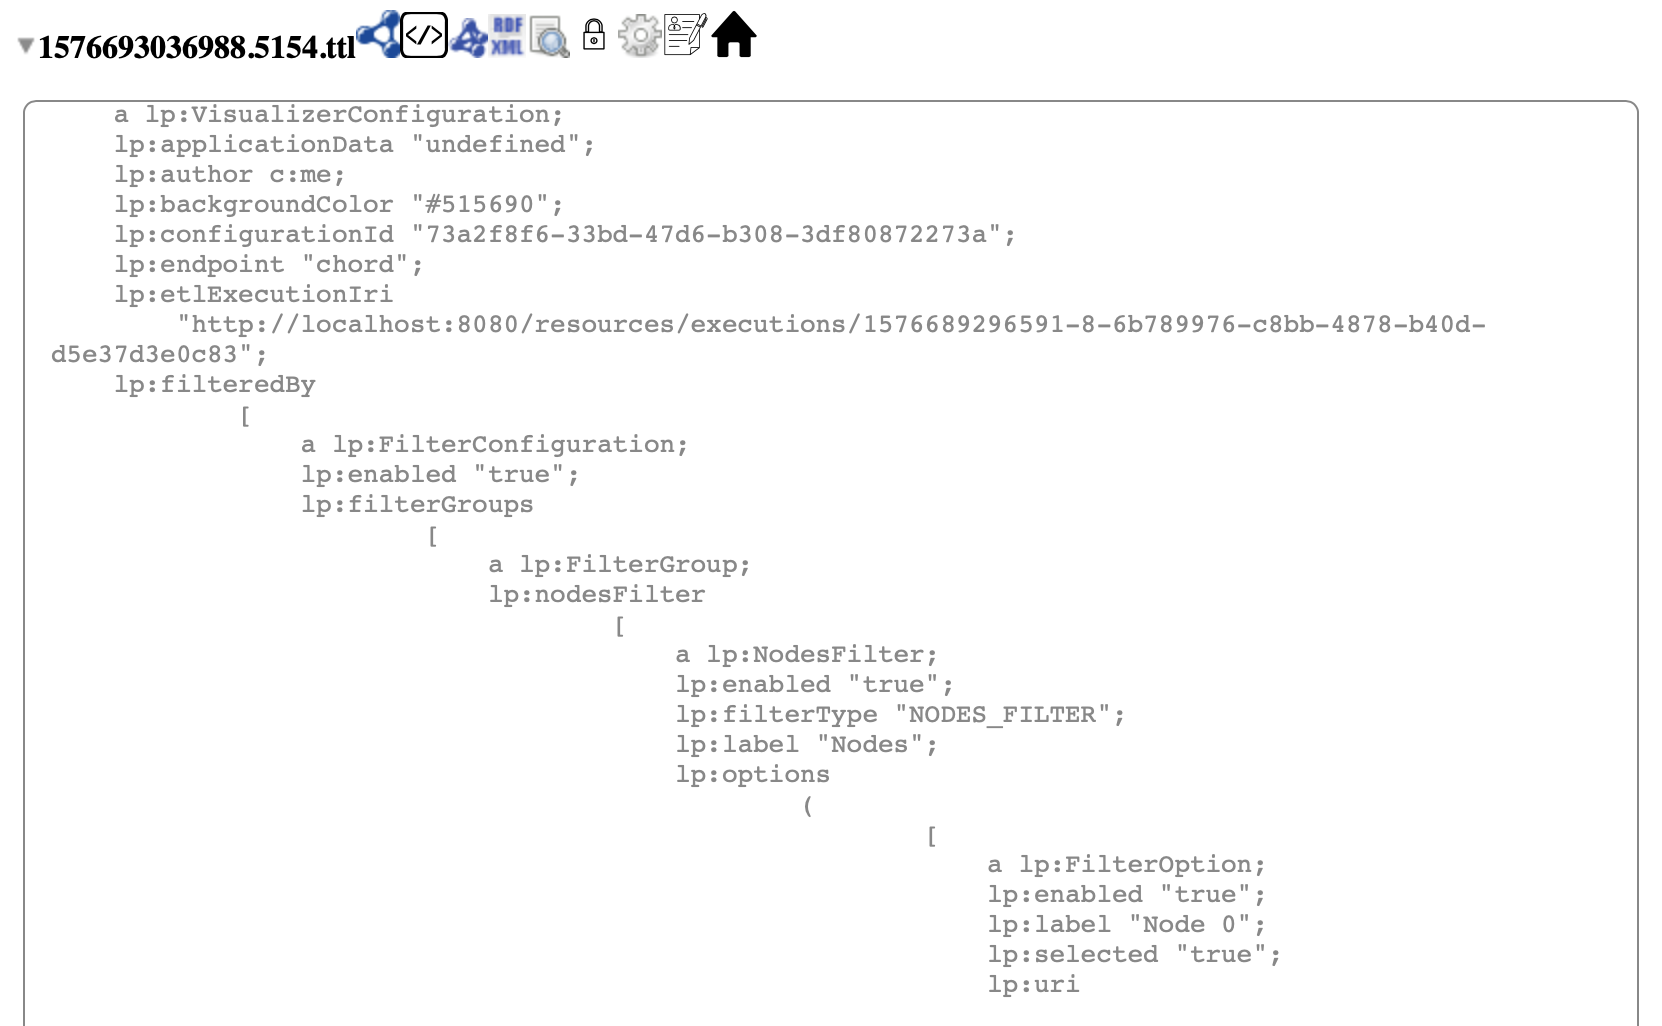
\includegraphics[width=0.8\linewidth]{solid_published_app_config.png}}
\caption{Published application configuration inside \solid{} POD.}
\label{fig:solid_published_app_config}
\end{figure}

\subsection{Sharing the Application}

As the final step of this user-story based interaction flow, John either embeds the application into his website or shares the link to his application with Bob. The screenshot on \autoref{fig:published_solid_application} demonstrates the resulting published application assembled from visualizer configuration stored in John's \solid{} POD as an RDF TTL resource. Additionally, Bob can access the webpage without creating an official profile inside the \lpa{} platform since it is publically available. 

\begin{figure}[h]
\centering
\fcolorbox{black}{white}{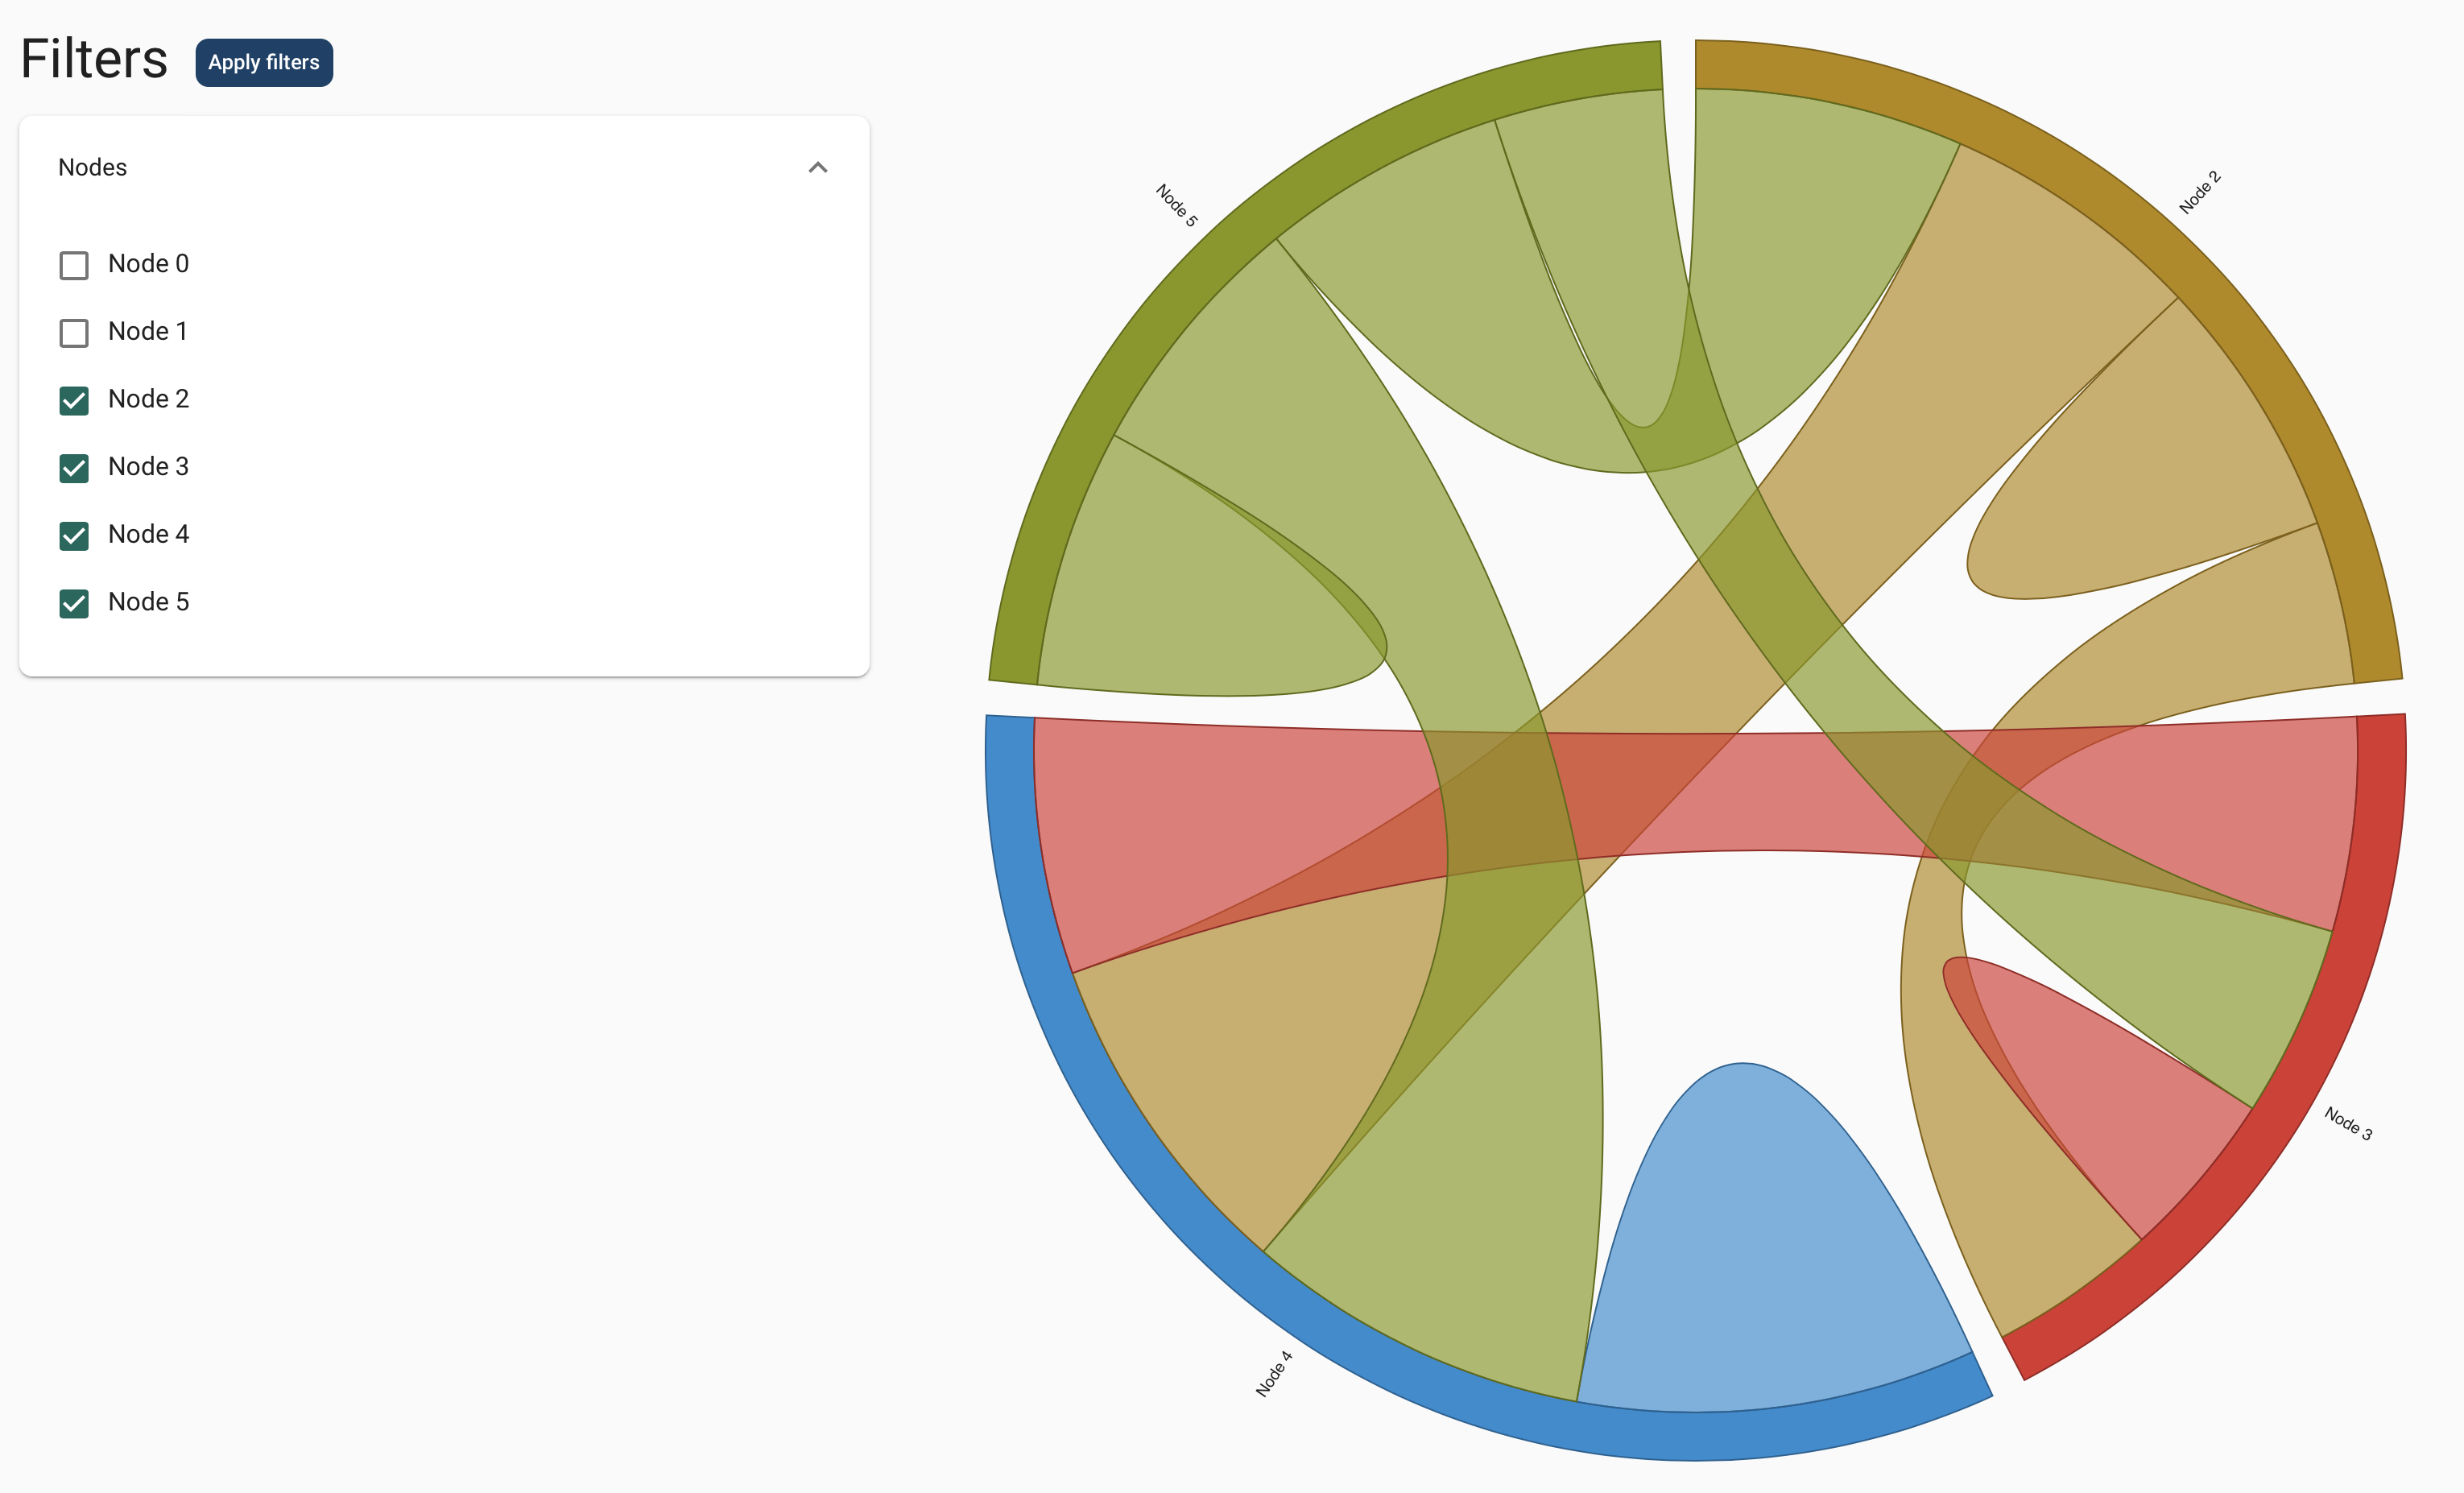
\includegraphics[width=0.8\linewidth]{published_solid_application.png}}
\caption{Published and publicly accessible application accessed via \textit{Share} URL.}
\label{fig:published_solid_application}
\end{figure}

To sum up, this section concludes the user-oriented documentation demonstrating the most basic interaction flow with \lpa{} platform using \lpas{} package and React Storage Components. 

\subsection{\lpa{} platform guide}

The user-story based guide demonstrated in the previous subsection only covered the essential functionality of \lpa{} made possible with the use of \lpas{} and \solid{}. Another important non-developer documentation resource is the \lpa{} platform documentation. That documentation was expanded with additional sections covering functionality, directly and indirectly, involving the interactions with \solid{} servers. Each section of the documentation is presented as a detailed video tutorial hosted on YouTube and can be described as follows:

\begin{itemize}
    \item \textit{Create, publish and embed your application} \footnote{\url{https://docs.applications.linkedpipes.com/tutorials/3.creating_applications/}} a video tutorial guiding users from start of application visualization creation to the finishing step where it is stored inside \solid{} POD, and a published URL is generated using the URI of the resource from the POD.
    \item \textit{Configuring application and filters} \footnote{\url{https://docs.applications.linkedpipes.com/tutorials/4.configuring_published_applications/}} a video tutorial demonstrating the configuration of published applications and editing of filter settings as described in \autoref{sssec:configuring_application_implementation}.
    \item \textit{Adding SOLID contacts, collaborative editing} \footnote{\url{https://docs.applications.linkedpipes.com/tutorials/5.adding_solid_contacts_sharing/}} a video tutorial demonstrated a process of adding new SOLID contacts in an instance of node-solid-server, and then demonstrates the process of sharing a published app with other user of the platform user as described in \autoref{ssssec:collaborative_sharing}.
    \item \textit{Managing platform and user settings} \footnote{\url{https://docs.applications.linkedpipes.com/tutorials/6.misc/}} a video tutorial demonstrating how to interact with the storage configuration and the \solid{} user profile settings popups. 
\end{itemize} 

More detailed and developer-oriented documentation is provided in consecutive chapters.

\section{Developer documentation}

The following section is intended for developers interested in a more in-depth overview of both \lpas{} package and React Storage Components implemented inside \lpa{} frontend codebase.

\subsection{Installation}

The following section will provide a set of guidelines covering various use-cases on trying out the \lpas{} package on a local machine. The installation process depends on two separate use-cases. First, it relies on simply trying to use the \lpas{} npm package. Second, relies on installing the whole \lpa{} platform to interact with \solid{}. 

\subsubsection{\lpas{} package}

It is important to note that this installation guide is not entirely generic for any \solid{} application. However, the \textit{AuthenticationManager} and \textit{FileManager} abstractions provide a generic functionality to be utilized in majority of \solid{} app development use-cases that involve authentication and interaction with resources inside the POD. The following prerequisites are required in order to install the \lpas{} package on a local machine:
\begin{itemize}
    \item \textit{Node.js v10.15.x and higher} \footnote{\url{https://nodejs.org/en/}}. The \lpas{} is distributed via npm, therefore a proper version of Node.js and a corresponding package manager are a required prerequisite. 
    \item \textit{yarn v1.19.1} \footnote{https://yarnpkg.com/en/}. Yarn is an alternative package manager similar to npm. Due to extensive usage of this package manager during development of \lpas{}, the author recommends it to be used as an alternative to npm.
\end{itemize}

\begin{listing}[H]    
\begin{minted}[breaklines,frame=single,framerule=1pt,bgcolor=LightGray]{bash}
$ yarn add linkedpipes-storage # if using yarn package manager
# or
$ npm install linkedpipes-storage # if using npm 
\end{minted}
\caption{Installing the \lpas{} package locally via yarn or npm.} 
\label{lst:installing_lpas}
\end{listing}

The code on \autoref{lst:installing_lpas} demonstrates the installation of the package at the folder from which the command is invoked. In other words, it is assumed that the package is being installed into a \solid{} based web app project. 

\subsubsection{\lpa{} platform}

Installation of entire \lpa{} platform is even more straightforward process in contrast with \lpas{} package. However, due to the complexity of components inside the platform, the recommended way to install it is by using Docker. Therefore, the only required prerequisite is the latest stable version of Docker and Docker Compose \footnote{\url{https://docs.docker.com}}. 

\begin{listing}[H]    
\begin{minted}[breaklines,frame=single,framerule=1pt,bgcolor=LightGray]{bash}
$ curl https://git.io/fjXIB -o lpa-cli.sh && chmod +x lpa-cli.sh && ./lpa-cli.sh --production-no-cloning
\end{minted}
\caption{Installing the \lpa{} platform locally using docker-compose.} 
\label{lst:installing_lpa_locally}
\end{listing}

The code snippet on \autoref{lst:installing_lpa_locally} demonstrates the local installation of entire \lpa{} platform using docker-compose, whose invocation is conveniently wrapped into a command line interface by \lpa{} developers.

\subsection{\lpas{} package}

The package is source codes are available at public GitHub repository \footnote{\url{https://github.com/aorumbayev/linkedpipes-storage}} and corresponding page on npm \footnote{\url{https://www.npmjs.com/package/linkedpipes-storage}}. The generic documentation on repository \textit{README}, as well as on a webpage at npm, includes the installation guide and a quick start on creating, editing, and deleting resources using a folder as an example. 

More detailed and developer oriented documentation is available on repository GitHub Page \footnote{\url{https://aorumbayev.github.io/linkedpipes-storage}}. The website is generated and published as a part of automated CI and CD pipeline demonstrated at \autoref{fig:lpas_ci_integration}. The documentation is generated using \texttt{typedoc} \footnote{\url{https://github.com/TypeStrong/typedoc}}, a documentation generator for TypeScript project. The codebase is annotated using \texttt{tsdoc} \footnote{\url{https://github.com/microsoft/tsdoc}}, an official TypeScript comment standard developed by Microsoft.

The typedoc documentation provides the overview of entire \lpas{} project codebase in the following order:
\begin{enumerate}
    \item \textit{Enumerations} description of all enumeration types in codebase.
    \item \textit{Classes} description of all class types in codebase.
    \item \textit{Interfaces} description of all interface types in codebase.
    \item \textit{Variables} description of all variable types in codebase.
    \item \textit{Functions} description of all function types in codebase.
\end{enumerate}

Every individual type is expanded into a detailed description of its sub-elements. For instance, every class type documentation is structured as follows:
\begin{enumerate}
    \item \textit{Constructors} description of all class constructors, input parameters and return values.
    \item \textit{Properties} description of all properties of the class, their types and inheritance hierarchy.
    \item \textit{Constructors} description of all class method, input parameters and return values.
\end{enumerate}

For more details, refer to the package documentation website listed in the footnote at the beginning of this section.

\subsection{Storage Components}

The Storage Components documentation is a part of \lpa{} documentation. Therefore the section will firstly provide a brief description of how the \lpa{} platform is documented and finally how the Storage Components documentation was integrated.

There are three main documentation sources provided by \lpa{} platform described as follows:
\begin{itemize}
    \item \textit{The platform documentation} \footnote{\url{https://docs.applications.linkedpipes.com}}, as mentioned and demonstrated earlier in \autoref{sssec:user_documentation_guides}, it contains non-developer oriented tutorials, introduces core concepts of the platform, and provides a detailed set of video tutorials demonstrating the available feature. This documentation was expanded by including interactions with storage components. The corresponding video tutorials were recorded to illustrate and guide users to use and interact with storage. The static webpage was generated using \texttt{hugo} framework \footnote{\url{https://gohugo.io}}.
    \item \textit{The frontend documentation} \footnote{\url{https://docs.frontend.applications.linkedpipes.com}} contains developer-oriented guideline over frontend components of the platform generated using \texttt{docz} \footnote{\url{https://www.docz.site}}. Provide the main installation, quick start, and interactive documentation of selected components of the platform. Each of the interactive components can be immediately forked into \texttt{codesandbox} environment \footnote{\url{https://codesandbox.io}} and tested in an online web IDE environment. 
    \item \textit{The backend documentation} \footnote{\url{https://docs.backend.applications.linkedpipes.com}} contains developer-oriented guideline over backend components of the platform generated using \texttt{orchid} \footnote{\url{https://orchid.run}}. No additional documentation for \lpas{} related code was added since no changes were required on the backend component side.
\end{itemize}

For references to a so-called \textit{Admin documentation} and information on hosting the \lpa{} instance using \lpas{} refer to project GitHub repository \footnote{\url{https://github.com/linkedpipes/applications}}. 

\subsubsection{Expanding frontend documentation}

As mentioned earlier in the section, the frontend documentation was created using docz framework, which relies on a special markdown syntax called \textit{MDX} \footnote{\url{https://mdxjs.com}}. It allows for combining the advantages of generic markdown syntax and JavaScript code snippets. Therefore, inside the frontend codebase, each component representing the individual platform webpage had an MDX file added, having the same name as the JSX component file. Later on, the docz framework automatically assembles the static HTML pages based on the declared MDX files describing components. 

The following Storage Components were added into general frontend documentation by implementing the corresponding MDX files:
\begin{itemize}
    \item \textit{StoragePage} represents a set of components rendered into a Storage Dashboard. The documentation includes the structure of stateful and stateless components that are associated with the webpage. The main properties passed to the components are also described. Lastly, a live instance of that webpage is rendered inside the documentation webpage, allowing developers to interact with the component.
    \item \textit{SettingsPage} represents both user profile and storage control settings pages. The documentation includes the structure of stateful and stateless components that are associated with the webpage and main properties used by those components. 
\end{itemize}

The frontend documentation also contains the dedicated section describing the Storage Components in general and provides several references to \solid{} toolset that was used as well as the \lpas{} package. For more details, refer to the package documentation website listed in the footnote at the beginning of this section.


